%%\chapter{Revisão da literatura}
\label{Fundamentacao}
%
%	\begin{flushright}
%		\textit{``O período de maior ganho em conhecimento e experiência
%		\\ é o período mais difícil da vida''.\\Dalai Lama}
%	\end{flushright}
%
%

Neste capítulo busca-se contextualizar o leitor dos fundamentos teóricos nos quais este trabalho se baseia, mais especificamente abordando de forma detalhada o funcionamento da técnica DTM. Além disso, as tecnologias utilizadas na realização desta pesquisa serão apresentadas de forma teórica, permitindo ao leitor assimilar seu funcionamento e assim melhor compreender sua aplicação prática descrita no capítulo \ref{Desenvolvimento}.

Para melhor compreensão, este capítulo é dividido em cinco seções. Na seção \ref{Fundamentacao:EstadoArte} é apresentado o estado da arte da técnica DTM. Na seção \ref{Fundamentacao:DTM} ocorre a demonstração de como funciona a técnica de memorização dinâmica de traces de forma teórica. Na seção \ref{Fundamentacao:DTMHardware} vemos uma adaptação da técnica para aplicação prática em hardware. Na seção \ref{Fundamentacao:LEON3} é apresentado o processador LEON3 juntamente com outras tecnologias auxiliares. Por fim, na seção \ref{Fundamentacao:FPGA} é explicado como funciona o FPGA, tecnologia para gravação de circuitos utilizada neste trabalho.

\section{Estado da Arte}
\label{Fundamentacao:EstadoArte}

Apesar de não ser tão difundida quanto outras técnicas, a memorização de computações anteriores tem sido alvo de alguns estudos na busca pelo aumento do desempenho de sistemas computacionais. Por ser um conceito amplo, existem margens para diversas aplicações diferentes, tanto em hardware quanto em software. Como exemplo pode ser citado o trabalho realizado por \cite{citron1998accelerating}, que utilizou a memorização em hardware para reduzir a latência média de unidades de multiplicação e divisão multiciclo. Devido ao foco no reuso de instruções dado a este trabalho, nesta seção serão apresentados rapidamente alguns trabalhos relacionados a esta aplicação de memorização.

Além de realizar um estudo sobre a repetição de instruções, \citeonline{sodani1997dynamic} propõe o uso da técnica de memorização para o reuso de instruções. Os quatro esquemas propostos fazem uso de uma unidade de memória denominada \textit{Reuse Buffer}. O esquema $S_{v}$ armazena e compara apenas os valores do conteúdo dos registradores utilizados na instrução, semelhantemente ao DTM. O esquema $S_{n}$ utiliza apenas o identificador do registrador e um bit de validade que é alterado quando os registradores indicados sofrem escrita. Os esquemas $S_{n+d}$ e $S_{v+d}$ buscam identificar dependências entre as instruções para permitir o reuso de conjuntos de instruções, algo parecido com o reuso de traces mas com entradas para instruções individuais indicando as dependências em vez da construção de uma entrada única para o trace. Todos esses esquemas permitem o reuso de instruções para carregar dados da memória.

\citeonline{gonzalez1999trace} apresenta uma forma teórica de reuso de traces completos, utilizando uma estrutura denominada \textit{Reuse Trace Memory}. Sua estratégia se assemelha à DTM porém inclui posições de memória nos contextos de entrada e saída, apesar que os problemas de consistência e latência gerados por esta inclusão não são adereçados. Além disso, não é especificado o comportamento da técnica em instruções de desvio, o que pode trazer efeitos colaterais indesejáveis considerando a ampla difusão do uso de estruturas que se baseiam em execuções anteriores para realizar a predição de desvios.

\citeonline{costa2001explorando} introduz a técnica de reuso explorada nas seções \ref{Fundamentacao:DTM} e \ref{Fundamentacao:DTMHardware}. Seu trabalho consiste em descrever uma maneira viável de explorar o reuso dinâmico de instruções a nível de hardware. Para isso se baseou na literatura mas apresentando inovações, permitindo por exemplo um reuso de sequências de instruções mais eficiente que \citeonline{sodani1997dynamic} porém tratando questões que poderiam tornar tal unidade impraticável diferentemente de \citeonline{gonzalez1999trace}, como a remoção do reuso de memória e o tratamento específico para instruções de desvio. Além disso foram realizados testes sobre a eficiência de tal técnica através de simulações de uma arquitetura superescalar com DTM incorporado.

\citeonline{pilla2003limits} introduz a RST, que é a execução especulativa aplicada à técnica DTM, realizando o reuso mesmo em condições onde nem todos os valores do contexto de entrada foram testados. Alterando a tabela de armazenamento de traces, a \tablet, e reutilizando partes do esquema de predição de desvios já presentes na arquitetura foi criada uma unidade que, para níveis de acerto de predição acima de 90\%, produziu ganhos de performance em relação à técnica DTM.

No trabalho de \citeonline{silva2006memorizacao} é demonstrada a técnica JDTM, que adapta a DTM para a utilização em máquinas Java. A natureza de máquina de pilha de uma arquitetura Java demanda que alterações sejam realizadas, já que os operandos, tanto de entrada como de saída, de uma instrução deixam de ser registradores específicos para serem posições relativas ao topo da pilha. Assim como em \citeonline{costa2001explorando}, resultados positivos foram obtidos na execução de \textit{benchmarks} em simulações da arquitetura com JDTM.

\citeonline{laurino2007reuso} expande a técnica RST para incluir o reuso de instruções de acesso à memória. A RSTm inclui uma nova tabela, a \tablel, para realizar o acompanhamento das instruções de manipulação de memória. Assim é paralelamente comparado o PC atual com a \tableg, \tablet\ e \tablel, reusando um trace ou uma instrução envolvendo ou não acessos à memória caso seja detectada redundância através de uma instância anterior armazenada.

%%%%%%%%%%%%%%%%%%%%%%%%%%%%%%%%%%%%%%%%%%
%%%%%%% TA MEIO ESQUISITO ESSE REF %%%%%%%
%%%%%%%%%%%%%%%%%%%%%%%%%%%%%%%%%%%%%%%%%%

Todos estes trabalhos citados anteriormente produzem seus resultados através de modelos teóricos ou simulações computacionais. Porém certos aspectos de um processador alterados ao inserir novas unidades não são facilmente detectados através de simulações, como discutido na seção \ref{Metodologia:Analise}. Por isso há a necessidade de realizar a implementação em hardware físico a fim de melhor avaliar essas outras características e validar a viabilidade prática do mecanismo DTM.

\section{Memorização dinâmica de traces}
\label{Fundamentacao:DTM}

A memorização dinâmica de traces é uma técnica que busca evitar a perda de tempo computacional reduzindo o número de execuções de instruções já executadas. Diferente de algumas técnicas de programação que exploram o reuso de computação a nível de software, a DTM trabalha a nível de hardware e identifica candidatos ao reuso de forma dinâmica. Essa identificação dinâmica se caracteriza por reutilizar instruções em qualquer ponto do programa, categorizando uma instrução ou sequência de instruções como redundante de acordo com os valores dos seus parâmetros de entrada, comparando-os aos de uma execução anterior \cite{costa2001explorando}.

Na figura \ref{Fig:ExemploDTM} vemos um exemplo do funcionamento de DTM em um fluxo de controle. Na figura, cada nó representa um instrução e as ligações entre os nós representam os possíveis caminhos de execução de um código. 

Em (a) é possível observar uma sequência de instruções que foram executadas pelo programa, com os nós em cinza claro simbolizando as instruções executadas enquanto os nós em branco os caminhos não tomados.

Em (b) temos em cinza escuro os nós que representam instruções redundantes executadas. Após a identificação dessas instruções, ocorre a construção do trace e a memorização deste.

Em (c) é representado como o fluxo de controle se comporta quando ocorre o reuso do trace. Como pode ser notado, as instruções identificadas como redundantes não são executadas. Ocorre então a escrita dos resultados gerados na execução memorizada e o desvio para a próxima instrução a ser executada que não pertence ao trace, considerando qualquer desvio que tenha sido tomado entre as instruções reusadas.

\begin{figure}
\label{Fig:ExemploDTM}
	\caption[Exemplo das etapas do processo de DTM em um fluxo de controle]{
	Exemplo do processo de DTM em um fluxo de controle: (a) Instruções executadas; (b) Instruções redundantes identificadas, memorização; (c) Fluxo de controle quando ocorre reuso do trace.}
	
	\centering
	\begin{multicols}{3}
		\begin{tikzpicture}[->,>=stealth,shorten >=1pt,auto,node distance=1cm,thick,main node/.style={fill=black!20,circle,draw,font=\sffamily}]
	
		\node[main node] (1) { };
		\node[main node] (2) [below of=1] { };
		\node[main node] (3) [below of=2] { };
		\node[main node, style={thin, fill=none}] (4) [below left of=3] { };
		\node[main node] (5) [below right of=3] { };
		\node[main node, style={draw=none, fill=none}] (erapraser6) [below left of=4] { };
		\node[main node] (6) [below left of=5] { };
		\node[main node, style={thin, fill=none}] (7) [below right of=5] { };
		\node[main node, style={thin, fill=none}] (8) [below right of=6] { };
		\node[main node] (9) [below left of=6] { };
		\node[main node, style={draw=none, fill=none}] (erapraser10) [below of=7] { };
		\node[main node, style={draw=none, fill=none}] (10) [below of=8] { };
		\node[main node] (11) [below of=9] { };
		\node[main node] (12) [below right of=11] { };
		\node[main node, style={thin, fill=none}] (13) [below left of=11] { };
		\node[main node] (14) [below of=12] { };
		\node[main node, style={draw=none, fill=none}] (15) [below of=13] { };
		\node[main node] (16) [below of=14] { };
		\node[main node] (17) [below left of=16] { };
		\node[main node, style={thin, fill=none}] (18) [below right of=16] { };
		\node[main node] (19) [below of=17] { };
		\node[main node, style={draw=none, fill=none}] (20) [below of=16] {};
		\node[main node, style={draw=none, fill=none}] (21) [below of=20] {};
		\node[main node, style={draw=none, fill=none}] (a) [below of=21] {(a)};
		
		\path[every node/.style={font=\sffamily\small}]
		(1) edge (2)
		(2) edge (3)
		(3) edge (4)
			edge (5)
		(4)	edge (erapraser6)
		(5) edge (6)
			edge (7)
		(6) edge (8)
			edge (9)
		(7) edge (erapraser10)
		(8) edge (10)
		(9) edge (11)
		(11)edge (12)
			edge (13)
		(12)edge (14)
		(13)edge (15)
		(14)edge (16)
		(16)edge (17)
			edge (18)
		(17)edge (19);
		
		\end{tikzpicture}
		
		%%%%%%%%%%%%%%%%%%%%%%%%%%%%%%%%%%%%%%%%%%%%%%%%%%%%%%%%%%%%%%%%%%
		

		\begin{tikzpicture}[->,>=stealth,shorten >=1pt,auto,node distance=1cm,thick,main node/.style={fill=black!50,circle,draw,font=\sffamily}]
		
		\node[main node, style={fill=black!20}] (1) { };
		\node[main node] (2) [below of=1] { };
		\node[main node] (3) [below of=2] { };
		\node[main node, style={thin, fill=none}] (4) [below left of=3] { };
		\node[main node] (5) [below right of=3] { };
		\node[main node, style={draw=none, fill=none}] (erapraser6) [below left of=4] { };
		\node[main node] (6) [below left of=5] { };
		\node[main node, style={thin, fill=none}] (7) [below right of=5] { };
		\node[main node, style={thin, fill=none}] (8) [below right of=6] { };
		\node[main node] (9) [below left of=6] { };
		\node[main node, style={draw=none, fill=none}] (erapraser10) [below of=7] { };
		\node[main node, style={draw=none, fill=none}] (10) [below of=8] { };
		\node[main node] (11) [below of=9] { };
		\node[main node] (12) [below right of=11] { };
		\node[main node, style={thin, fill=none}] (13) [below left of=11] { };
		\node[main node] (14) [below of=12] { };
		\node[main node, style={draw=none, fill=none}] (15) [below of=13] { };
		\node[main node] (16) [below of=14] { };
		\node[main node] (17) [below left of=16] { };
		\node[main node, style={thin, fill=none}] (18) [below right of=16] { };
		\node[main node, style={fill=black!20}] (19) [below of=17] { };
		\node[main node, style={draw=none, fill=none}] (20) [below of=16] {};
		\node[main node, style={draw=none, fill=none}] (21) [below of=20] {};
		\node[main node, style={draw=none, fill=none}] (b) [below of=21] {(b)};
		
		\path[every node/.style={font=\sffamily\small}]
		(1) edge (2)
		(2) edge (3)
		(3) edge (4)
		edge (5)
		(4)	edge (erapraser6)
		(5) edge (6)
		edge (7)
		(6) edge (8)
		edge (9)
		(7) edge (erapraser10)
		(8) edge (10)
		(9) edge (11)
		(11)edge (12)
		edge (13)
		(12)edge (14)
		(13)edge (15)
		(14)edge (16)
		(16)edge (17)
		edge (18)
		(17)edge (19);
		
		\end{tikzpicture}
		
		%%%%%%%%%%%%%%%%%%%%%%%%%%%%%%%%%%%%%%%%%%%%%%%%%%%%%%%%%%%%%%%%%%
		
		
		\begin{tikzpicture}[->,>=stealth,shorten >=1pt,auto,node distance=1cm,thick,main node/.style={fill=black!50,circle,draw,font=\sffamily}]
		
		\node[main node, style={fill=black!20}] (1) { };
		\node[main node] (2) [below of=1] { };
		\node[main node] (3) [below of=2] { };
		\node[main node, style={thin, fill=none}] (4) [below left of=3] { };
		\node[main node] (5) [below right of=3] { };
		\node[main node, style={draw=none, fill=none}] (erapraser6) [below left of=4] { };
		\node[main node] (6) [below left of=5] { };
		\node[main node, style={thin, fill=none}] (7) [below right of=5] { };
		\node[main node, style={thin, fill=none}] (8) [below right of=6] { };
		\node[main node] (9) [below left of=6] { };
		\node[main node, style={draw=none, fill=none}] (erapraser10) [below of=7] { };
		\node[main node, style={draw=none, fill=none}] (10) [below of=8] { };
		\node[main node] (11) [below of=9] { };
		\node[main node] (12) [below right of=11] { };
		\node[main node, style={thin, fill=none}] (13) [below left of=11] { };
		\node[main node] (14) [below of=12] { };
		\node[main node, style={draw=none, fill=none}] (15) [below of=13] { };
		\node[main node] (16) [below of=14] { };
		\node[main node] (17) [below left of=16] { };
		\node[main node, style={thin, fill=none}] (18) [below right of=16] { };
		\node[main node, style={fill=black!20}] (19) [below of=17] { };
		\node[main node, style={draw=none, fill=none}] (20) [below of=16] {};
		\node[main node, style={draw=none, fill=none}] (21) [below of=20] {};
		\node[main node, style={draw=none, fill=none}] (c) [below of=21] {(c)};
		
		\path[every node/.style={font=\sffamily\small}]
		(1) edge (2)
		%(2) edge (3)
		(3) edge (4)
		edge (5)
		(4)	edge (erapraser6)
		(5) edge (6)
		edge (7)
		(6) edge (8)
		edge (9)
		(7) edge (erapraser10)
		(8) edge (10)
		(9) edge (11)
		(11)edge (12)
		edge (13)
		(12)edge (14)
		(13)edge (15)
		(14)edge (16)
		(16)edge (17)
		edge (18)
		(17)edge (19);
		
	    \draw 
	    (2.west)
	    -- ++(left:4.5em) 
	    |- (19.west);
		
		\end{tikzpicture}
	\end{multicols}

\legend{Fonte: elaborada pelo autor}
\end{figure}

\subsection{Identificação e memorização de traces}
\label{Fundamentacao:DTM:Identificacao}

A primeira etapa do processo de DTM é a identificação de traces. Traces são conjuntos sequenciais de instruções válidas redundantes e que não possuem efeitos colaterais. Instruções são consideradas redundantes quando, dado um determinado conjunto de entradas, a instrução produzirá sempre o mesmo resultado. Exemplos de instruções redundantes e sem efeitos colaterais incluem instruções lógicas e aritméticas e de desvio condicional e incondicional. Instruções que manipulam a memória primária e que executam sub-rotinas do sistema não são redundantes e possuem efeitos colaterais, portanto não serão constituintes de um trace. No caso da arquitetura SPARC também foram consideradas não redundantes as instruções que manipulam as janelas de registradores, já que adicionaram uma complexidade muito grande à criação e armazenamento de traces.

Operações envolvendo ponto-flutuante possuem a mesma caracterização quanto à redundância e causalidade de efeitos colaterais que as instruções citadas acima. Por exemplo, instruções aritméticas com ponto-flutuante são redundantes enquanto a manipulação de memória envolvendo-os não. Porém, como \citeonline{gabbay1996speculative} observa, instruções de ponto flutuante costumam ter baixa localidade espacial, o que no caso da construção de uma unidade de DTM as torna indesejáveis, por adicionarem complexidade desnecessária tendo em vista o baixo retorno causado por sua inclusão. Isso não impede que a técnica de memorização seja empregada em operações de ponto-flutuante para aumentar seu desempenho, como demonstrado por \citeonline{citron1998accelerating}.

Após a identificação do trace, se dá o processo de memorização. A memorização consiste em armazenar as informações necessárias para permitir a identificação de uma oportunidade de reuso de um trace, além de garantir que o circuito seja capaz de gerar corretamente as saídas necessárias e realizar um desvio para a próxima instrução a ser executada.



\subsection{Reuso de traces}
\label{Fundamentacao:DTM:Reuso}

O reuso de um trace ocorre quando este é redundante e possui uma instância memorizada equivalente ao que deve ser executado. Essas instâncias são equivalentes quando possuem a mesma sequência de instruções e o mesmo contexto de entrada.

O contexto de entrada é definido como o conjunto de valores utilizados no trace cuja origem é externa ao trace. De forma análoga, o contexto de saída são os valores gerados internamente ao trace e que estão disponíveis para uso externo ao término deste.

Como exemplo, tomemos um trace para o pseudocódigo demonstrado na figura \ref{Fig:ExemploContexto1}. Em um trace gerado após a execução desse código, os valores contidos em $a$, $b$ e $c$ são utilizados internamente antes de terem seus valores definidos no próprio trace, compondo então o contexto de entrada.

\begin{figure}[!h]
	\label{Fig:ExemploContexto1}
	\caption[Exemplo de pseudocódigo]{
		Exemplo de pseudocódigo.}
	
		\begin{algorithmic}
			\STATE $c \leftarrow c + a$
			\STATE $x \leftarrow c + b$
			\IF{$x \le 5$}
			\STATE $y \leftarrow x * 2$
			\ELSE
			\STATE $x \leftarrow x + 1$
			\ENDIF
		\end{algorithmic}
	\legend{Fonte: elaborada pelo autor}
\end{figure}

Suponhamos os valores de entrada como $a = 1$, $b = 2$ e $c = 3$. Com esses valores as instruções armazenadas no trace resultante se assemelhariam com o trace representado na figura \ref{Fig:ExemploContexto2}\footnote{Estariam inclusas no trace também as instruções de comparação e desvio responsáveis pelo desvio condicional, mas por terem formato e efeitos relativos à arquitetura foram omitidas para maior clareza no exemplo.}. 
%. Estariam inclusas no trace também as instruções de comparação e desvio responsáveis pelo desvio condicional, mas por terem formato e efeitos relativos à arquitetura foram omitidas para maior clareza no exemplo.

\begin{figure}[!h]
	\label{Fig:ExemploContexto2}
	\caption[Exemplo de trace para o pseudocódigo da figura \ref{Fig:ExemploContexto1}]{
		Exemplo de trace para o pseudocódigo da figura \ref{Fig:ExemploContexto1}.}
	
	\begin{algorithmic}
		\STATE $c \leftarrow c + a$
		\STATE $x \leftarrow c + b$
		\STATE $x \leftarrow x + 1$
	\end{algorithmic}
	\legend{Fonte: elaborada pelo autor}
\end{figure}

Com os valores do contexto de entrada contidos no parágrafo anterior, o contexto de saída deste trace é $c = 4$ e $x = 7$. Assim, sempre que os valores do contexto de entrada se igualarem a esses ao entrar no trace, não há necessidade de execução das instruções, ocorrendo então a escrita do contexto de saída diretamente. Como essas instruções não possuem efeito colateral, esse processo é transparente para o programa sendo executado.

É possível então observar a importância da memorização correta do trace. Ainda analisando o pseudocódigo da figura \ref{Fig:ExemploContexto1}, caso o contexto de entrada seja $a = 1$, $b = 2$ e $c = 1$, o contexto de saída é $c = 2$, $x = 4$ e $y = 8$. O trace gerado para essa execução difere do trace descrito anteriormente, tanto nas instruções contidas como nos resultados gerados, de forma que o reuso do trace impróprio pode levar a aplicação que está executando a produzir resultados incorretos.

\section{DTM em hardware}
\label{Fundamentacao:DTMHardware}

Na seção \ref{Fundamentacao:DTM} é explanado o funcionamento da técnica DTM de forma abstrata, sem detalhar como implementar em hardware um mecanismo capaz de executar tal tarefa. Esta seção apresenta uma possível implementação, descrita por \citeonline{costa2001explorando}.

A implementação de \citeonline{costa2001explorando} tem como alvo um processador com ISA MIPS I, uma ISA do tipo RISC tal qual a ISA SPARC, se assemelhando em muitas características ao processador LEON3 utilizado neste trabalho. Assim, a implementação apresentada nesta seção é adaptada para se adequar à ISA e desenho do LEON3.

Para armazenamento das informações relevantes ao reuso de um trace será utilizada uma unidade de memória denominada \tablet. Essa unidade de memória será organizada como uma tabela, na qual cada linha corresponde a um trace armazenado. Também é utilizada uma tabela para o armazenamento de informações sobre instruções individuais, denominada \tableg. Esta será utilizada para o reuso de instruções isoladas, enquanto aquela para o reuso de blocos de instruções sequenciais.

\subsection{A unidade \tableg}
\label{Fundamentacao:DTMHardware:TableG}

Como descrito anteriormente, o primeiro passo do processo de DTM é a identificação de instruções redundantes. Para que o reuso dessas instruções possa ser feito é necessário que as instâncias executadas sejam armazenadas em alguma estrutura, de forma que quando for identificada a redundância o resultado prévio possa ser prontamente utilizado.

Para cumprir este papel, foi projetada uma unidade de memória para armazenar uma tabela, denominada \tableg. A \tableg\ tem como função armazenar instâncias anteriores e permitir a leitura de resultados. Para que esses valores possam ser lidos e gravados de forma eficiente, essa tabela foi projetada tendo em cada linha uma instância de uma instrução redundante e em cada coluna um campo que deve ser armazenado.

\begin{figure}
	\label{Fig:MemoTableG}
	\caption[Representação da tabela \tableg]{
		Representação da tabela \tableg.}
	\begin{center}
		%A famosa gambiarra ataca novamente
		\newcommand{\tabela}[1]{
			\multicolumn{1}{|c|}{$#1$}
		}
		\begin{tabular}{*{8}{c}}
			tamanho em bits & $32$ & $32$ & $32$ & $32$ & $1$ & $1$ & $1$ \\
			\cline{2-8}
			& \tabela{pc} & \tabela{sv1} & \tabela{sv2} & \tabela{res/targ} & \tabela{jmp} & \tabela{brc} & \tabela{btaken} \\
			\cline{2-8}
			& \multicolumn{7}{c}{\vdots} \\
			\cline{2-8}
			& \tabela{pc} & \tabela{sv1} & \tabela{sv2} & \tabela{res/targ} & \tabela{jmp} & \tabela{brc} & \tabela{btaken} \\
			\cline{2-8}
		\end{tabular}
	\end{center}
	\legend{Fonte: elaborada pelo autor}
\end{figure}

Na figura \ref{Fig:MemoTableG} pode ser vista a distribuição dos bits na \tableg. Abaixo é definido o significado dos valores a serem estocados em cada campo da tabela:

\begin{itemize}
	\item $pc$: Responsável por armazenar o valor do contador de programa quando a instrução foi executada. Esse valor nada mais é que o endereço de memória onde está localizada a instrução.
	\item $sv1$: Armazena o valor do primeiro parâmetro passado para a instrução.
	\item $sv2$: Armazena o valor do segundo parâmetro passado para a instrução.
	\item $res/targ$: Campo onde é salvo o resultado da computação realizada, seja o resultado de uma instrução lógica, aritmética ou o endereço para um desvio.
	\item $jmp$: Caso a instrução seja um desvio incondicional será setado em $1$. Caso contrário estará em $0$.
	\item $brc$: Caso a instrução seja um desvio condicional será setado em $1$. Caso contrário estará em $0$.
	\item $btaken$: Caso a instrução seja um desvio condicional e tenha sido tomado, será setado em $1$. Caso contrário, não tendo sido tomado, estará em $0$. Caso não seja um desvio condicional seu valor é indeterminado.
\end{itemize}

Colocando esses valores armazenados em \tableg\ no contexto da técnica DTM, o campo $pc$ é utilizado para identificar a qual instrução pertence aquela instância armazenada. Como é necessário o armazenamento do campo $pc$ para identificação, não há razão para armazenar a tabela de outra forma que não completamente associativa. Os valores de $sv1$ e $sv2$ compõe o contexto de entrada de uma única instrução, podendo esta fazer uso de apenas um ou ambos de acordo com seu formato. Em $res/targ$ temos o contexto de saída da instrução.

Os três campos de um bit servem para identificar como deve ser utilizado o resultado. Caso os três tenham valor $0$, $res/targ$ é copiado para o registrador de destino indicado na instrução. Caso $jmp$ seja $1$, o valor de $res/targ$ é somado ao registrador de programa, o PC, realizando assim um desvio incondicional. Caso $brc$ esteja ativo a instrução é um desvio condicional, e o valor de $res/targ$ é somado ao PC caso $btaken$ também esteja ativo. Independentemente do valor de $btaken$, caso $brc$ esteja ativo ambos os bits serão utilizados para atualizar a unidade de predição de desvios, caso este exista.

\subsection{A unidade \tablet}
\label{Fundamentacao:DTMHardware:TableT}

Analogamente à \tableg, a \tablet\ tem como objetivo armazenar dados de instâncias de instruções armazenadas afim de permitir o reuso destas em execuções futuras. Porém, diferentemente daquela, esta armazena informações sobre traces, sendo então responsável por guardar todas as informações necessárias para o reuso de um conjunto de duas ou mais instruções redundantes.

O projeto da \tablet, apesar de compartilhar características com a estrutura da \tableg, deve ser adaptado para que o armazenamento de informações sobre um trace completo possam ser utilizadas de forma a identificar um trace redundante e reutilizá-lo de forma transparente à aplicação utilizando a unidade de processamento. 

A \tablet\ é então também uma unidade de memória completamente associativa organizada em forma tabular na qual cada linha representa um trace, ou seja uma instância de execução de uma sequência de instruções, e cada coluna um campo necessário para identificação ou reuso correto deste trace. A descrição destes campos, que podem ser vistos na figura \ref{Fig:MemoTableT}, segue abaixo:

\begin{itemize}
	\item $pc$: Onde é guardado o endereço de memória da primeira instrução do trace, usado para identificação de candidatos a reuso.
	\item $npc$: Armazena o endereço de memória da próxima instrução a ser executada. Após o reuso de um trace é necessário um desvio para a instrução subsequente, sendo então utilizado o valor de $npc$ para o cálculo desse desvio.
	\item $icr$: Identifica quais registradores pertencem ao contexto de entrada.
	\item $icv$: Armazena os valores do contexto de entrada, contido nos registradores indicados pelo campo $icr$.
	\item $ocr$: Identifica quais registradores pertencem ao contexto de saída.
	\item $ocv$: Armazena os valores do contexto de saída, contido nos registradores indicados pelo campo $ocr$.
	\item $bmask$: Máscara na qual cada bit em nível alto indica a presença de um desvio no trace.
	\item $btaken$: Máscara que armazena para cada desvio indicado em $bmask$ se ele foi tomado ou não.
\end{itemize}

\begin{figure}
	\label{Fig:MemoTableT}
	\caption[Representação da tabela \tablet]{
		Representação da tabela \tablet.}
	\begin{center}
		%A famosa gambiarra ataca novamente novamente
		\newcommand{\tabela}[1]{
			\multicolumn{1}{|@{ }c@{ }|}{#1}
		}
		
		\newcommand{\tabelatripla}[2]{
			\tabela{$#1_{1}$} & \tabela{\hdots} & \tabela{$#1_{#2}$}
		}
		
		\tiny
		\begin{tabular}{*{21}{c}}
			tamanho em bits & $32$ & $32$ & \multicolumn{3}{c}{$5 * N_{1}$} & \multicolumn{3}{c}{$32 * N_{1}$} & \multicolumn{3}{c}{$5 * N_{2}$} & \multicolumn{3}{c}{$32 * N_{2}$} & \multicolumn{3}{c}{$1 * B$} & \multicolumn{3}{c}{$1 * B$} \\
			\cline{2-21}
			& \tabela{$pc$} & \tabela{$npc$} & \tabelatripla{icr}{N_{1}} & \tabelatripla{icv}{N_{1}} & \tabelatripla{ocr}{N_{2}} & \tabelatripla{ocv}{N_{2}} & \tabelatripla{bmask}{B} & \tabelatripla{btaken}{B}  \\
			\cline{2-21}
			\multicolumn{21}{c}{\vdots} \\
			\cline{2-21}
			& \tabela{$pc$} & \tabela{$npc$} & \tabelatripla{icr}{N_{1}} & \tabelatripla{icv}{N_{1}} & \tabelatripla{ocr}{N_{2}} & \tabelatripla{ocv}{N_{2}} & \tabelatripla{bmask}{B} & \tabelatripla{btaken}{B}  \\
			\cline{2-21}
		\end{tabular}
		\normalsize
		
	\end{center}
	\legend{Fonte: elaborada pelo autor}
\end{figure}

A figura \ref{Fig:MemoTableT} também indica o uso de três parâmetros configuráveis: $N_{1}, N_{2}, B  \in \mathbb{Z}$. O significado de cada um é explicado a seguir.

$N_{1}$ define quantos registradores podem pertencer ao contexto de entrada de um trace. Caso o para continuar a construção do trace esse seja necessário mais registradores, a construção será encerrada. 

Com uso bastante semelhante a $N_{1}$, $N_{2}$ limita a quantidade de registradores no contexto de saída. \citeonline{costa2001explorando} utiliza $N_{1}, N_{2} \mid N_{1} = N_{2}$, mas isso não é necessário para o funcionamento correto do DTM. Em aplicações que os traces comumente possuem mais valores no contexto de saída que no de entrada é desejável criar a tabela tal que $N_{1} < N_{2}$. Da mesma forma, caso o contexto de entrada costume ser maior que o de saída, podem ser escolhidos valores para os quais $N_{1} > N_{2}$. Cabe ao projetista ajustar a unidade para melhor se adaptar as características dos traces nela armazenados, atingindo assim melhor desempenho e evitando desperdício de memória.

Por fim, $B$ indica a quantidade máxima de instruções de desvio que serão armazenadas em um trace. Os valores armazenados em $bmask$ e $btaken$ são utilizados para atualizar as unidades de predição de desvio. Caso a aplicação envolva muitas instruções de desvio, aumentar o valor de $B$ aumentará o tamanho máximo dos traces armazenados, permitindo o reuso de mais instruções com uma única entrada.

Esses parâmetros devem ser definidos no momento da construção do hardware. A existência desses se deve ao fato de não interferirem no bom funcionamento da técnica mas influenciar os resultados. A medida que se aumenta o valor dos parâmetros o tamanho máximo dos traces também aumenta, o que pode causar um ganho de desempenho dependendo da aplicação sendo executada. Porém, esses valores são diretamente proporcionais à quantidade de memória necessária para o armazenamento, aumentando a área de chip e o custo do hardware resultante.


\subsection{Construção e reuso}
\label{Fundamentacao:DTMHardware:Integracao}

Para construção de um trace são utilizados dois mapas de contexto e um \textit{buffer} temporário. Esse \textit{buffer} possui o mesmo formato de uma linha da \tablet, enquanto os mapas possuem um bit para cada registrador, totalizando 32 bits.

Quando uma instrução redundante é identificada se inicia a construção do trace. O valor do registrador PC é inserido no \textit{buffer} no campo $pc$, enquanto seu valor somado 4 no $npc$. Para cada registrador pertencente ao contexto de entrada, o respectivo bit na máscara de contexto de entrada é posta em nível alto. Caso o bit estivesse em $0$, o número do registrador e seu valor são inseridos no \textit{buffer}. O mesmo se aplica ao mapa de contexto de saída, com a diferença que caso haja duas escritas em um registrador o valor em $ocv$ é atualizado, o que não ocorre no contexto de entrada. Caso a instrução a ser executada seja um desvio, os devidos bits são escritos nas máscaras do \textit{buffer} temporário. 

Para cada instrução subsequente, caso seja redundante, o campo $npc$ recebe o valor do registrador PC mais quatro, enquanto os outros valores são inseridos e atualizados como descrito anteriormente. Caso a instrução não seja redundante o \textit{buffer} é escrito em uma entrada da \tablet\ e os valores do \textit{buffer} e dos mapas são zerados.

Paralelamente, para cada instrução é verificado em \tableg\ e \tablet\ se existem entradas para as quais valor de $pc$ equivale ao do registrador PC. Para as que são encontradas, é verificado então o contexto de entrada. Os registradores indicados pelo campo $icr$ tem seus valores lidos do banco de registradores e comparados com os valores de $icv$ para cada entrada identificadas de \tablet. Já para \tableg, os registradores indicados na própria instrução tem seus valores comparados com os campos $sv1$ e $sv2$. Caso haja um trace em \tablet\ no qual todos os registradores passem neste teste, ele então é reusado. Caso não haja um trace mas haja um instrução em \tableg, ela então é reusada. Caso contrário, a instrução é executada normalmente.

\section{O LEON3}
\label{Fundamentacao:LEON3}

O LEON3 é um processador 32-bit baseado na arquitetura SPARC V8 atualmente mantido pela Cobham Gaisler. Disponibilizado sob a licensa GPL, o código-fonte é na linguagem VHDL e implementado utilizando \textit{generics}, o que permite a configuração dos parâmetros que definem algumas características do processador \cite{grlibmanual}.

O LEON3 possui um banco de registradores com suporte para 2 a 32 janelas. Cada janela tem acesso a 32 registradores:

\begin{itemize}
	\item \textit{Global}: 8 registradores acessíveis por todas as janela. Utilizados para armazenamento de valores globais. Registradores 0 a 7.
	\item \textit{Out}: 8 registradores acessíveis pela janela atual e pela próxima janela. Utilizados para passagem de parâmetros e recebimento de valores de retorno. Registradores 8 a 15.
	\item \textit{Local}: 8 registradores acessíveis somente pela janela atual. Utilizados para variáveis locais e valores temporários. Registradores 16 a 23.
	\item \textit{In}: 8 registradores acessíveis pela janela atual e pela janela anterior. Utilizados para recebimento de parâmetros e retorno de valores. Registradores 24 a 31.
\end{itemize}

A janela atual é determinada pelo \textit{Current Window Pointer}, um contador de 5 bits contido no registrador \textit{Processor State Register}. O contador é incrementado com a instrução RETT e decrementado com a SAVE. O objetivo dessas janelas é agilizar a troca de contexto, permitindo a mudança de vários registradores para um valor anterior em menos instruções \cite{sparcmanual}.

\begin{figure}
	\label{Fig:Leon3Interno}
	\caption[Diagrama de blocos interno do LEON3]{
		Diagrama de blocos interno do LEON3.}
	\begin{center}
		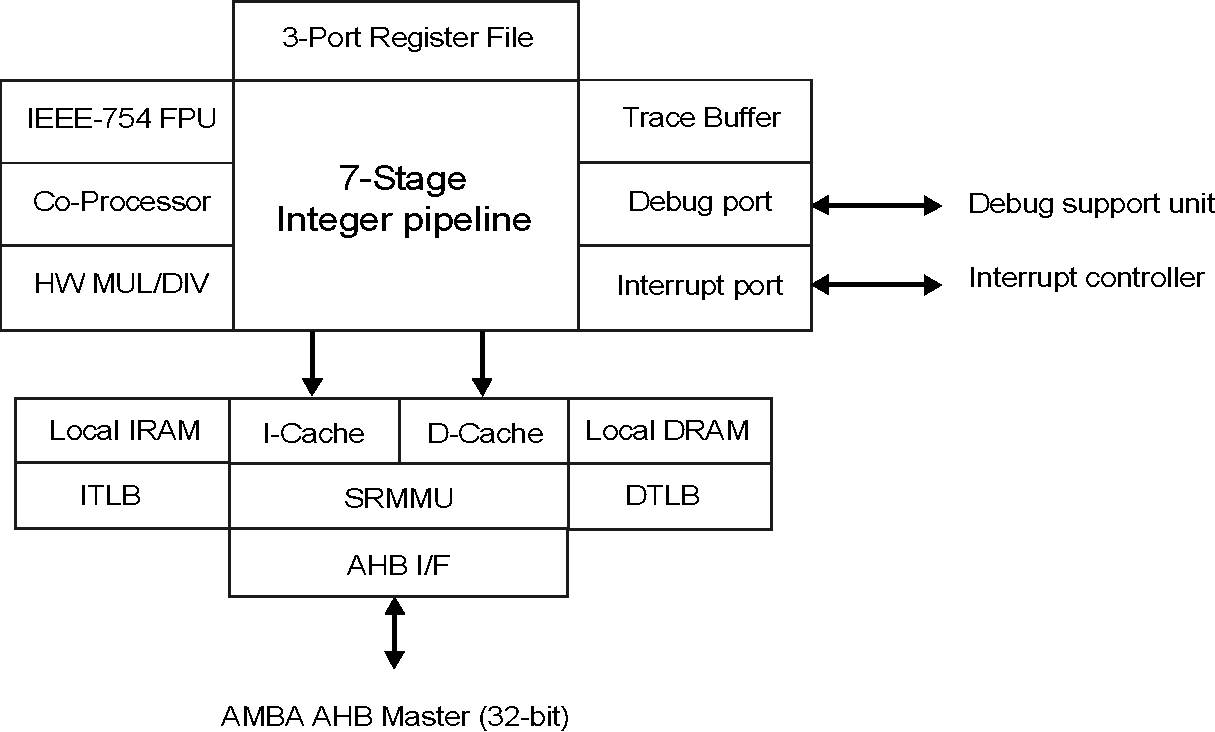
\includegraphics[width=\linewidth]{fig/leon3interno.pdf}
	\end{center}
	\legend{Fonte: \cite{leondatasheet}}
\end{figure}

Ao configurar o sistema antes da compilação do código-fonte também é possível optar pela inclusão de uma unidade de processamento de ponto-flutuante. Duas unidades estão disponíveis, a GRFPU e a GRFPU-Lite, ambas se adequando ao padrão IEEE-754.

Além dessas unidades, como demonstrado na figura \ref{Fig:Leon3Interno} são incluídas outras unidades como suporte a depuração, multiplicadores e divisores em hardware, entre outros \cite{grlibmanual}.


\begin{figure}
	\label{Fig:Leon3Externo}
	\caption[Diagrama de blocos de um sistema utilizando o GRLIB]{
		Diagrama de blocos de um sistema utilizando o GRLIB.}
	\begin{center}
		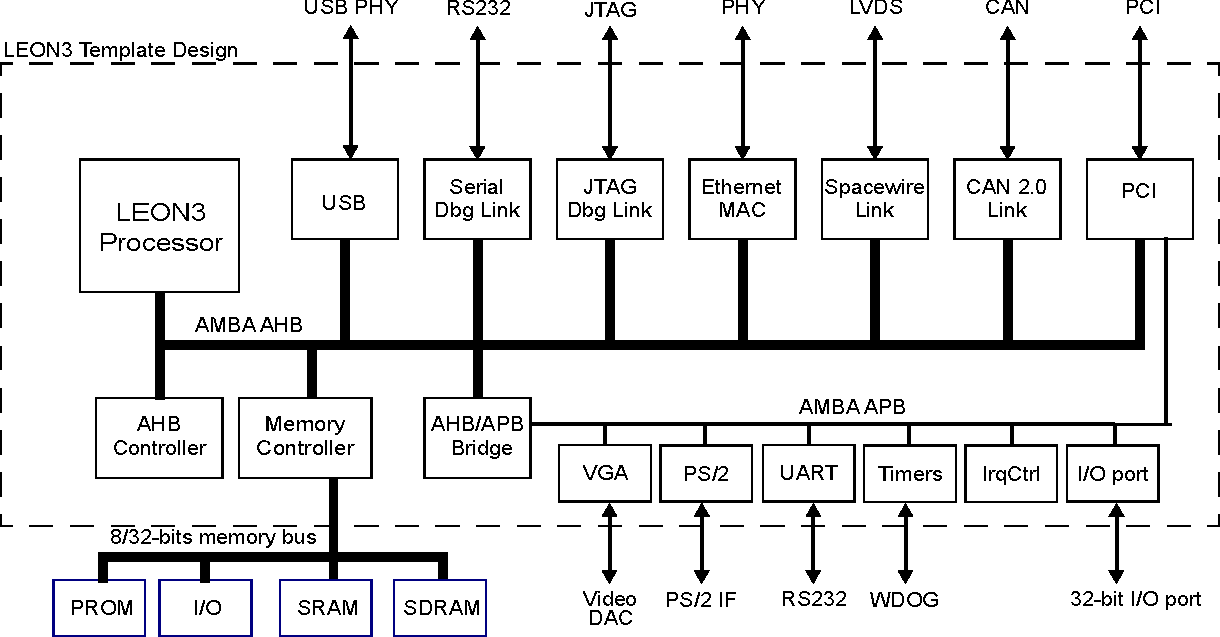
\includegraphics[width=\linewidth]{fig/leon3externo.pdf}
	\end{center}
	\legend{Fonte: \cite{grlibmanual}}
\end{figure}

A unidade de inteiros, que lida com as instruções que não são de ponto-flutuante na arquitetura SPARC, é organizada em um pipeline de 7 estágios:

\begin{enumerate}
	\item FE (\textit{Instruction Fetch}): A instrução é buscada na cache de instruções. Caso haja um \textit{miss} a devida instrução é buscada no barramento.
	\item DE (\textit{Decode}): A instrução é decodificada. O endereço de desvio é calculado.
	\item RA (\textit{Register Access}): Os registradores utilizados são lidos do banco ou de alguma unidade de \textit{fowarding}.
	\item EX (\textit{Execute}): Operações lógicas e aritméticas são executadas. Endereços de acesso de memória e de retorno de chamada são calculados.
	\item ME (\textit{Memory}): Caso a instrução requisite, é feito um acesso à cache de dados. Na ocorrência de um \textit{miss} ou de uma escrita (o tratamento de escritas é \textit{write-through}) o comando é enviado ao barramento principal.
	\item XC (\textit{Exception}): Tratamento de excessões e interrupções.
	\item WR (\textit{Write}): O resultado da operação lógica ou aritmética é escrito no banco de registradores.
\end{enumerate}

As memórias caches são separadas para instruções e dados. Seus tamanhos, formatos e associatividades são configuráveis. A presença de uma MMU para auxiliar o gerenciamento de memória é opcional. As requisições de memória são realizadas para o barramento AHB.

Como pode ser visto na figura \ref{Fig:Leon3Externo}, um sistema GRLIB utiliza uma barramento segundo o padrão AMBA 2.0. O processador é conectado ao barramento AHB, juntamente com o controlador de memória e outras unidades como entradas para JTAG, USB, Ethernet, entre outros. Também está conectado neste barramento um controlador ponte para o APB. O APB é responsável por controle dos periféricos, como temporizadores e portas de entrada e saída de dados  \cite{grlibmanual}.


\section{\textit{Field-Programmable Gate Array}}
\label{Fundamentacao:FPGA}

Devido a sua versatilidade e relativo baixo custo, decidiu-se por utilizar a tecnologia de FPGA para realização dos testes de hardware. Para produção de poucas unidades, tecnologias ASIC possuem um custo por unidade muito maior que o uso de FPGA, além desta oferecer a possibilidade de realização de modificações no hardware depois de pronto, o que é impossível naquela \cite{chu2006rtl}.

Nesta seção será apresentado brevemente o funcionamento de um circuito de FPGA. A intenção é permitir ao leitor a compreensão que mesmo sendo diferente de um circuito impresso, um circuito gravado em FPGA compartilhará de quase todas as suas características apesar de sua diferente configuração.

%%%%%%%%%%%%%%%%%%%%%%%%%%%%%%%%%%%%%%%%%%%%%
%%%% <REESCREVER>

Como dito anteriormente, chips de FPGA são programáveis e, apesar de serem mais caros que um CI de produção em massa, é muito mais barato para poucas unidades a gravação em FPGA que a criação de um CI específico. Porém, apesar de se mostrarem mais lentos que circuitos usando tecnologias ASIC, os circuitos em FPGA possuem um comportamento semelhante a suas a estes, já que placas de FPGA foram feitas para emularem as conexões entre elementos lógicos contidas em um circuito ASIC.
Isso os torna ideais para prototipação e testes de hardware, já que é possível testar de forma barata e versátil a funcionalidade e características de um determinado circuito. 

Além disso, a comparação de modelos gravados em circuito utilizando uma tecnologia como FPGA permite tirar conclusões para esses modelos, mesmo que sejam utilizados posteriormente de outras maneiras. Cabe ressaltar que a comparação de valores entre projetos de circuito deve considerar a proporcionalidade causada pela diferença de tecnologias \cite{tanenbaum2009organizacao}.

%%%% </REESCREVER>
%%%%%%%%%%%%%%%%%%%%%%%%%%%%%%%%%%%%%%%%%%%%%

Um circuito de FPGA é composto principalmente de \textit{Lookup Tables} e interconexões programáveis. A replicação desses componentes e a possibilidade de programá-los independentemente dá ao FPGA uma capacidade de criar diversos circuitos lógicos de acordo com os valores dados.

Uma LUT é uma pequena unidade de memória que armazena valores determinados pelo hardware a ser gerado. Ao combinar os pinos de endereçamento formando uma posição de memória, o valor gravado é lido e colocado nos pinos de saída. Dessa forma uma LUT é capaz de simular o funcionamento de qualquer função lógica que possua um número de entradas menor ou igual seu número de pinos de endereçamento. Combinando as entradas e saídas de unidades que contém uma LUT de forma programável permite a emulação de uma infinidade de circuitos lógicos, limitados apenas pela quantidade de elementos lógicos contidos no chip utilizado \cite{tanenbaum2009organizacao}.

Neste trabalho foi feito uso do dispositivo Altera Cyclone II. Neste as LUT possuem 16 posições de memória, com quatro pinos para endereçamento. Essas LUT estão contidas em unidades chamadas \textit{Logic Elements}, que são a unidade lógica mínima na arquitetura. Uma LE também possui um registrador programável e suporte para sinal de \textit{feedback}, \textit{clock} e \textit{clear}. Por estarem agrupadas em conjuntos denominados \textit{Logic Array Blocks}, cada LE possui um sinal de entrada \textit{carry in} e um sinal de saída \textit{carry out}, facilitando o uso de conjuntos de LE para operações aritméticas \cite{altera2007cyclone}.